 \section{Bayes-Formel}
\textbf{Satz 2.2}:\\
Seien A,B $\subset \Omega$ zwei Ereignisse mit $\mathds{P}[A] \neq 0, \mathds{P}[B] \neq 0$. Dann gilt:
$$\mathds{P}[B \vert A] = \dfrac{\mathds{P}[A\vert B] * \mathds{P}[B]}{\mathds{P}[A]}$$
\textbf{Beweis}: Linke Seite = $\mathds{P}[B\vert A] = \dfrac{\mathds{P}[B \cap A]}{\mathds{P}[A]}$\smallskip\\
Rechte Seite = $\dfrac{\mathds{P}[A \vert B] * \mathds{P}[B]}{\mathds{P}[A]} = \dfrac{\mathds{P}[A \cap B]}{\mathds{P}[A]} \qed$\\\\
\textbf{Beispiel 1: (Population Personen: krank und gesund)}\medskip\\
1\% der Population ist krank.
\begin{tabbing}
	Schnelltest: \= Bei einer Kranken Person mit Wahrscheinlichkeit 90\% positiv.\\
	\> Bei einer gesunden Person mit Wahrscheinlichkeit 20\% positiv
\end{tabbing}
Eine gesunde Person wurde positiv getestet.\\
Wahrscheinlichkeit, dass diese Person krank ist?\smallskip
\begin{tabbing}
\textbf{Lösung 1}:\medskip\\
$\Omega$ = Population \hspace{1cm} \= $B_1 = $ ''Person ist krank''\\
\> $B_2 = B_1^C = $ ''Person ist gesund''
\end{tabbing}
A = ''Person wurde positiv getestet''\\
Aufgabenstellung: $\mathds{P}[B_1] = 0,01 \Rightarrow \mathds{P}[B_2] = 1-0,01=0,99$
\begin{enumerate}
	\item $\mathds{P}[A \vert B_1] = 0,9$
	\item $\mathds{P}[A \vert B_2] = 0,2$
\end{enumerate}
$\mathds{P}[B_1\vert A] = ?$\\
Bayes-Formel: $\mathds{P}[B_1 \vert A] \overset{\text{Bayes}}{=} \dfrac{\mathds{P}[A\vert B_1] * \mathds{P}[B_1]}{\mathds{P}[A]} \overset{\text{totale Wkeit}}{=} $\smallskip\\$
\dfrac{\mathds{P}[A \vert B_1]*\mathds{P}[B_1]}{\mathds{P}[A \vert B_1]*\mathds{P}[B_1]+\mathds{P}[A\vert B_2]*\mathds{P}[B_2]} = \dfrac{0,9*0,01}{0,9*0,01+0,2*0,99}= 0,043$\medskip\\
$\mathds{P}[B_2 \vert A] = 1- \mathds{P}[B_1 \vert A ] = 1-0,043$\\\\
\textbf{Lösung 2}:\\ 
$\mathds{P}[A] = 0,01*0,9+0,99*0,2 = 0,207$\medskip\\
$\mathds{P}[\text{krank}\vert \text{positiv getestet}]= \dfrac{0,01*0,9}{0,01*0,9+0,99*0,2} = 0,043$\\\\\\\\
\textbf{Lösung 3}:\\
Laplace-Experiment mit $\Omega = \{\text{KP, KN, GP, GN}\}$\\
P(KP) = 0,9*0,01 \hspace{2cm} P(GP) = 02*0,99\\
P(KN) = 0,1*0,01 \hspace{2cm} P(GN) = 0,8*0,99\smallskip\\
A = ''Person positiv'' = \{KP, GP\}\\
$B_1$ = ''Person krank'' =  \{KP, KN\} 
$$\mathds{P}[B_1\vert A] = \dfrac{\mathds{P}[B_1 \cap A]}{\mathds{P}[A]} = \dfrac{P(\text{KP})}{P(\text{KP})+P(\text{GP})} = ...$$\medskip\\
\textbf{Beispiel 2: (2 Jungen Problem)}\\
Im Nachbarhaus: Familie mit 2 Kindern.\\
Sie beobachten: Im Garten spielt ein Junge.\\
Wkeit, dass das $\underbrace{\text{andere Kind auch ein Junge}}_\text{d.h. beide sind Jungen}$ ist = ?\smallskip\\
\textbf{Lösung}:\\
Grundmenge: $\Omega = \{\text{MM1, MM2, MJ1, MJ2, JM1, JM2, JJ1, JJ2}\}$\\
MM1 = Beides Mädchen, erste Kind im Garten\smallskip\\
B = ''Im Garten spielt ein Junge'' = \{MJ2, JM1, JJ1,JJ2\}\\
A = ''Beide Kinder sind Jungen'' = \{JJ1, JJ2\} \hspace{1cm} $A\cap B = $\{JJ1,JJ2\}\medskip\\
$\mathds{P}[A\vert B] = \dfrac{\mathds{P}[A \cap B]}{\mathds{P}[B]} = \dfrac{2/8}{4/8} = 0.5$\bigskip\\
\textbf{Beispiel 3: (Ziegenproblem)}
\begin{tabbing}
	3 Türen \hspace{1cm} \= Hinter einer Tür $\rightarrow$ Auto\\
	\> Hinter den beiden anderen $\rightarrow$ Ziegen
\end{tabbing}
Sie zeigen auf Tür 1. (Tür 1 bleibt aber geschlossen)\\
Moderator öffnet eine der beiden anderen Türen $\rightarrow$ Ziege.\\
Sie dürfen bei Tür 1 bleiben oder wechseln. Was ist besser?\smallskip\\
Aufgabenstellung ist unvollständig. Wir machen die Annahme: Moderator weiß, wo das Auto steht und will das Auto nicht zeigen.\newpage
\textbf{Lösung}: \\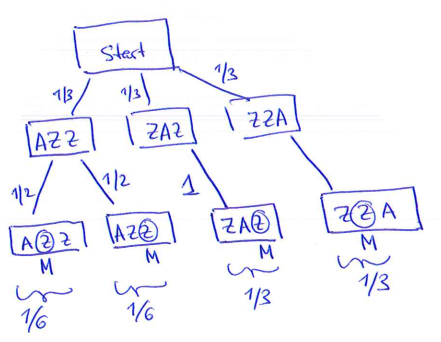
\includegraphics[width=0.6\textwidth]{img/ziege.PNG}\\
$\Omega =$ \{A\textbf{Z}Z, AZ\textbf{Z},ZA\textbf{Z},Z\textbf{Z}A\}\ \hspace{ 1cm} Dick geschrieben: Vom Moderator  gewählt \medskip\\
p(A\textbf{Z}Z) = $\frac{1}{3}*\frac{1}{2}$\smallskip\\
p(AZ\textbf{Z}) = $\frac{1}{3}*\frac{1}{2}$\smallskip\\
p(ZA\textbf{Z}) = $\frac{1}{3}*1$\smallskip\\
p(Z\textbf{Z}A) = $\frac{1}{3}*1$\medskip\\
$\mathds{P}[\text{Auto hinter Tür 1}] $ = p(A\textbf{Z}Z)+p(AZ\textbf{Z}) = $\frac{1}{6}+\frac{1}{6}=\frac{1}{3}$\\
$\mathds{P}[\text{Türwechsel führt zum Erfolg}]$ = p(ZA\textbf{Z})+p(Z\textbf{Z}A) = $\frac{1}{3}+\frac{1}{3}= \frac{2}{3}$\medskip\\
\textbf{Also wechseln!}

